\documentclass[UTF8,a4paper,8pt]{ctexbook} 

 \usepackage{graphicx}%学习插入图
 \usepackage{verbatim}%学习注释多行
 \usepackage{booktabs}%表格
 \usepackage{geometry}%图片
 \usepackage{amsmath} 
 \usepackage{amssymb}
 \usepackage{listings}%代码
 \usepackage{xcolor}  %颜色
 \usepackage{enumitem}%列表格式
 \usepackage{hyperref}
 \CTEXsetup[format+={\flushleft}]{section}


\geometry{left=1.6cm,right=1.8cm,top=2cm,bottom=1.7cm} %设置文章宽度

\pagestyle{plain} 		  %设置页面布局
\author{郑华}
\title{C++  服务器案例学习笔记}
 %代码效果定义
 \definecolor{mygreen}{rgb}{0,0.6,0}
 \definecolor{mygray}{rgb}{0.5,0.5,0.5}
 \definecolor{mymauve}{rgb}{0.58,0,0.82}
 \lstset{ %
 	backgroundcolor=\color{white},   % choose the background color
 	basicstyle=\footnotesize\ttfamily,        % size of fonts used for the code
 	%stringstyle=\color{codepurple},
 	%basicstyle=\footnotesize,
 	%breakatwhitespace=false,         
 	%breaklines=true,                 
 	%captionpos=b,                    
 	%keepspaces=true,                 
 	%numbers=left,                    
 	%numbersep=5pt,                  
 	%showspaces=false,                
 	%showstringspaces=false,
 	%showtabs=false,        
 	columns=fullflexible,
 	breaklines=true,                 % automatic line breaking only at whitespace
 	captionpos=b,                    % sets the caption-position to bottom
 	tabsize=4,
 	commentstyle=\color{mygreen},    % comment style
 	escapeinside={\%*}{*)},          % if you want to add LaTeX within your code
 	keywordstyle=\color{blue},       % keyword style
 	stringstyle=\color{mymauve}\ttfamily,     % string literal style
  	frame=single,					%tb top and bottom; L left double line
  	xleftmargin=.06\textwidth, 
  	%xrightmargin=.1\textwidth,
 	rulesepcolor=\color{red!20!green!20!blue!20},
 	% identifierstyle=\color{red},
 	language=c++,
 }

\begin{document}          %正文排版开始
 	\maketitle
 	\tableofcontents
\chapter{开源-muduo-0.8.2}	
	 \section{架构图}
		 \begin{figure}[h]
		 	\centering
		 	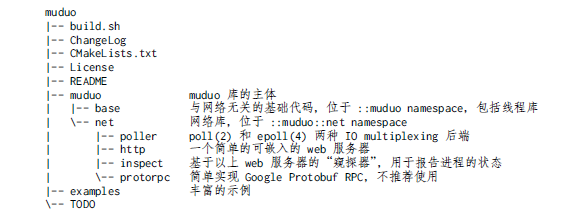
\includegraphics[scale = 0.7]{muduo.png}
		 	\caption{架构图}
		 \end{figure}
 
	 \section{参考}
		 代码架构:见muduo 参考手册,net 文件夹下
		 
		 博客:\url{http://www.cppblog.com/Solstice/default.html?page=3}
		 
			 \url{https://www.oschina.net/question/28_61182}
			
\chapter{开源-libevent-1.4}
	\section{参考}
		代码架构:见参考手册,net 文件夹下
	
\chapter{开源-lighthttpd-1.4.15}
	\section{架构图}
		\begin{figure}[h]
			\centering
			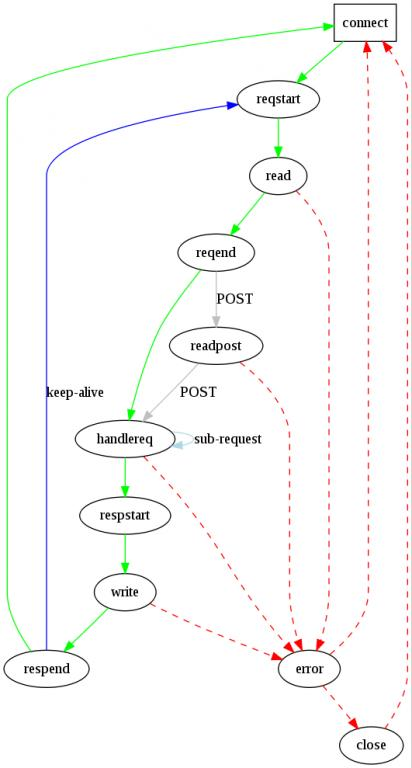
\includegraphics[scale = 0.5]{lighttpd.jpg}
			\caption{架构图}
		\end{figure}
\chapter{开源-nginx-0.5.38}
	\section{架构}
		\begin{figure}[h]
			\centering
			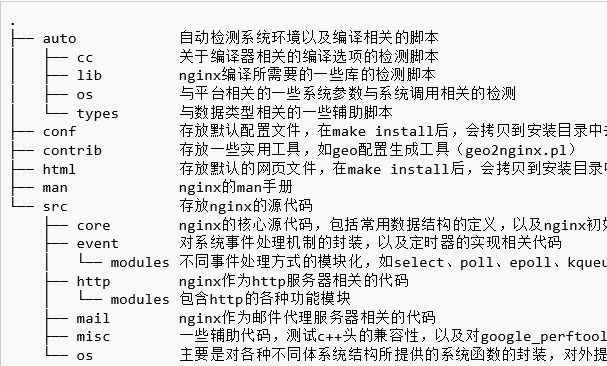
\includegraphics[scale = 0.7]{nginx.png}
			\caption{架构图}
		\end{figure}
	\section{参考}
		代码架构:\url{http://tengine.taobao.org/book/chapter_09.html}

\chapter{游戏服务器 - 戴汉水}    
	\section{经验学习}
		 \subsection{\#ifdef .. 编译选择}
		 
		 \subsection{string 和 wstring 相互转换}
		 
		 \subsection{GBK 和 UTF8 的相互变换}
		 
		 \subsection{boost 智能指针}
		 
		 \subsection{游戏服务器种类}
		 数据库服务器, 游戏服务器, 登陆服务器, battle 服务器
		 
		 \subsection{enum 枚举的使用}
		 
		 \subsection{按模块编码,而不是头文件与cpp 文件}有点像java包的概念,像包一样的分解程序,分解成lib,然后调用,继承
		 
\newpage
	\section{错误记录}
		\subsection{错误	204	error LNK2001: 无法解析的外部符号} 
		\verb|"__declspec(dllimport)| 
		
		\verb|class std::basic_ostream<char,struct std::char_traits<char> >| 
		
		\verb|& __cdecl std::endl(class std::basic_ostream<char,struct std::char_traits<char> > &)"| 
		
		\subparagraph{解决办法}
		VS20xx:
		
		项目、属性、链接器、常规、附加库目录:填写附加依赖库所在目录 分号间隔多项
		
		项目、属性、链接器、输入、附加依赖项:填写附加依赖库的名字.lib 空格或分号间隔多项


\chapter{游戏服务器2 - 戴汉水}
	\section{经验}
	
		\subsection{设置自己的 解决方案目录结构}:\url{http://www.360doc.com/content/13/0422/10/8251840_280065154.shtml}
	
	
		\subsection{学会程序 跟踪,与Debug}
	\section{错误记录}
		\subsection{Error MSB3073 代码9009}:
		
		\subsection{Error fatal error LNK1104: cannot open file 'atlsd.lib'}:\url{http://blog.csdn.net/hsluoyc/article/details/46312293}
		
		貌似是 2008以前版本用的库有个 atlsd.lib, 由于atlsd.lib在高版本VS中也不存在,因此只好用其Release版本代替,经测试可以使用。没有安装高版本VS的同学可以留言索取atls.lib。
		
		
		\subsection{Project : error PRJ0019: 工具从"正在执行预生成事件..."}
			配置属性-生成事件-预编译事件或生成后事件-命令行,删除命令行内容即可
			
			
		\subsection{subwcrev 不是内部或外部命令,也不是可运行的程序}:
			svn 命令: 该版本visual studio  未安装SVN 版本控制器, 导致的错误
			
		\subsection{resource 文件目录如果打不开}请检查是不是不存在.rc文件,或.rc文件多了后缀如.rc.in
				
\chapter{游戏解决方案的搭建}
	\section{DLL动态库}
	
	\section{调用DLL}
	
	\section{调用DLL中的头文件,但其实不是}	


\chapter{Others}
	\section{线程池}多线程技术主要解决处理器单元内多个线程执行的问题,它可以显著减少处理器单元的闲置时间,增加处理器单元的吞吐能力。
	
		线程池的好处就在于线程复用,一个任务处理完成后,当前线程可以直接处理下一个任务,而不是销毁后再创建,非常适用于连续产生大量并发任务的场合。
			
		\url{http://wenku.baidu.com/view/f0bd6127ccbff121dd36831a.html}
	
		\subsection{核心思想} 假设一个服务器完成一项任务所需时间为:T1 创建线程时间,T2 在线程中执行任务的时间,T3 销毁线程时间。
		
		如果:T1 + T3 远大于 T2,则可以采用线程池,以提高服务器性能。
		
		\textbf{线程池技术正是关注如何缩短或调整T1,T3时间的技术,从而提高服务器程序性能的},它把T1,T3分别安排在服务器程序的启动和结束的时间段或者一些空闲的时间段,这样在服务器程序处理客户请求时,不会有T1,T3的开销了。
		
		除此之外,线程池能够减少创建的线程个数。通常线程池所允许的并发线程是有上界的,如果同时需要并发的线程数超过上界,那么一部分线程将会等待。而传统方案中,如果同时请求数目为2000,那么最坏情况下,系统可能需要产生2000个线程。尽管这不是一个很大的数目,但是也有部分机器可能达不到这种要求。  
		
		因此线程池的出现正是着眼于减少线程池本身带来的开销。线程池采用预创建的技术,在应用程序启动之后,将立即创建一定数量的线程(N1),放入空闲队列中。这些线程都是处于阻塞Suspended)状态,不消耗CPU,但占用较小的内存空间。当任务到来后,缓冲池选择一个空闲线程,把任务传入此线程中运行。当N1个线程都在处理任务后,缓冲池自动创建一定数量的新线程,用于处理更多的任务。在任务执行完毕后线程也不退出,而是继续保持在池中等待下一次的任务。当系统比较空闲时,大部分线程都一直处于暂停状态,线程池自动销毁一部分线程,回收系统资源。  
		
		基于这种预创建技术,线程池将线程创建和销毁本身所带来的开销分摊到了各个具体的任务上,执行次数越多,每个任务所分担到的线程本身开销则越小,不过我们另外可能需要考虑进去线程之间同步所带来的开销。
		\subsection{组成部分}
			\subparagraph{1.线程池管理器 ThreadPool}用于创建并管理线程池,包括 创建线程池,销毁线程池,添加新任务
			
			\subparagraph{2.工作线程 PoolWorker}线程池中线程,在没有任务时处于等待状态,可以循环的执行任务
			
			\subparagraph{3.任务接口 Task}每个任务必须实现的接口,以供工作线程调度任务的执行,它主要规定了任务的入口,任务执行完后的收尾工作,任务的执行状态等
			
			\subparagraph{4.任务队列 taskQueue}用于存放没有处理的任务。提供一种缓冲机制。
		
		\subsection{实现}
			\subparagraph{C++}\url{http://wenku.baidu.com/view/a4cc1093daef5ef7ba0d3c3a.html}
			
			\subparagraph{Boost}\url{http://www.oschina.net/code/snippet_170948_18231}
		
		
\end{document} 
 		    